% Main file. Compile with pdfLaTeX, BibTeX, pdfLaTeX, pdfLaTeX.
% In a clean directory the embedded bibliography creates reference.bib.
% In an existing project merge the entries below into its reference.bib.
\begin{filecontents*}{reference.bib}
@article{liu2026clutter,
 author={Rang Liu and Peishi Li and Ming Li and A. Lee Swindlehurst},
 title={Clutter-Aware Integrated Sensing and Communication: Models, Methods, and Future Directions},
 journal={arXiv:2602.10537}, year={2026},
 note={\href{https://arxiv.org/abs/2602.10537}{Author manuscript, version 2}}}
@article{nguyen2024hybrid,
 author={Nhan Thanh Nguyen and Ly V. Nguyen and Nir Shlezinger and Yonina C. Eldar and A. Lee Swindlehurst and Markku Juntti},
 title={Joint Communications and Sensing Hybrid Beamforming Design via Deep Unfolding},
 journal={IEEE Journal of Selected Topics in Signal Processing}, year={2024},
 note={\href{https://doi.org/10.1109/JSTSP.2024.3463403}{Publisher version}}}
\end{filecontents*}
\documentclass[11pt,letterpaper]{article}
\usepackage[T1]{fontenc}
\usepackage{lmodern,amsmath,amssymb,graphicx,tikz}
\usepackage[margin=0.82in]{geometry}
\usetikzlibrary{arrows.meta,positioning,shapes.geometric}
\usepackage[colorlinks=true,linkcolor=blue!45!black,citecolor=blue!45!black,urlcolor=blue!45!black]{hyperref}
\hypersetup{pdftitle={Fixed-array near-field ISAC with limited clutter observations},pdfauthor={Muneef Mohammed}}
\newcommand{\A}{\mathbf A}\newcommand{\W}{\mathbf W}\newcommand{\Q}{\mathbf Q}
\newcommand{\R}{\mathbf R}\newcommand{\uu}{\mathbf u}\newcommand{\qq}{\mathbf q}
\newcommand{\CN}{\mathcal{CN}}\newcommand{\tr}{\operatorname{tr}}
\newcommand{\scnr}{\operatorname{SCNR}}
\setlength{\parindent}{0pt}\setlength{\parskip}{4pt}\raggedbottom
% BEGIN EDITABLE FIGURE
\newcommand{\systemdrawing}{%
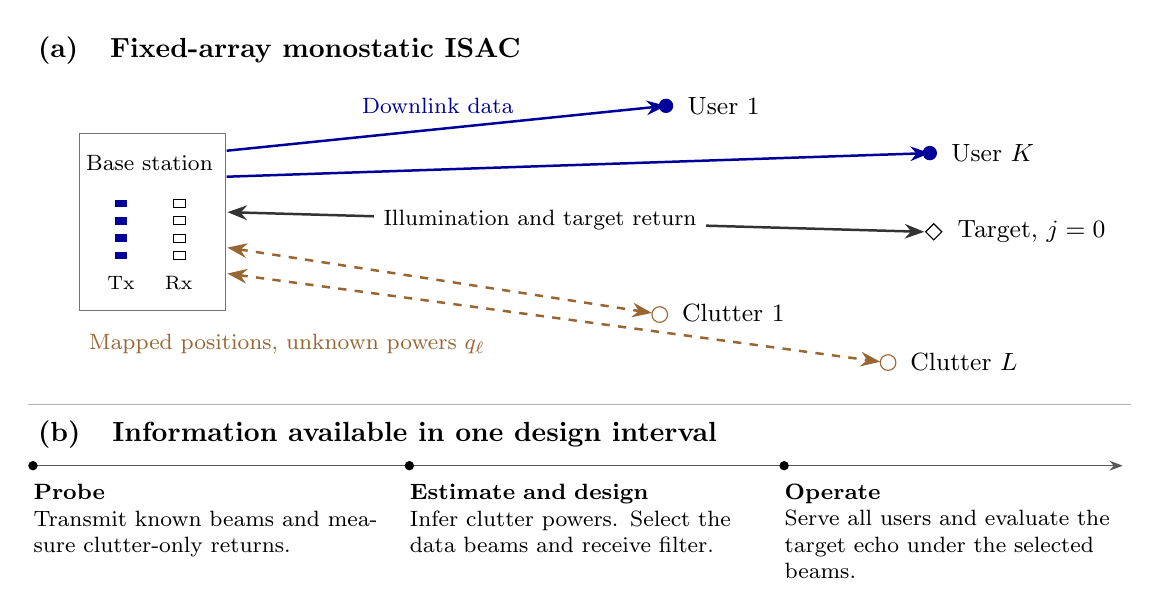
\begin{tikzpicture}[x=1cm,y=1cm,font=\small,>=Stealth,
 link/.style={->,line width=.9pt,blue!60!black},
 targetlink/.style={<->,line width=.9pt,black!80},
 clutterlink/.style={<->,dashed,line width=.9pt,brown!80!black},
 stage/.style={anchor=north west,align=left,font=\footnotesize,text width=4.55cm,inner sep=0pt}]
\node[anchor=west,font=\bfseries] at (0,4.75) {(a)\quad Fixed-array monostatic ISAC};
\draw[black!55] (.65,1.45) rectangle (2.5,3.7);
\node[align=center,font=\footnotesize] at (1.54,3.32) {Base station};
\foreach \y in {2.1,2.32,2.54,2.76}{\fill[blue!60!black] (1.1,\y) rectangle ++(.15,.1);\draw (1.85,\y) rectangle ++(.15,.1);}
\node[font=\scriptsize] at (1.18,1.8) {Tx};\node[font=\scriptsize] at (1.91,1.8) {Rx};
\coordinate (u1) at (8.1,4.05);\coordinate (uk) at (11.45,3.45);
\draw[link] (2.52,3.48)--(u1);\draw[link] (2.52,3.15)--(uk);
\fill[blue!60!black] (u1) circle (2.6pt);\fill[blue!60!black] (uk) circle (2.6pt);
\node[anchor=west] at (8.25,4.05) {User 1};\node[anchor=west] at (11.6,3.45) {User $K$};
\node[font=\footnotesize,blue!60!black] at (5.2,4.05) {Downlink data};
\draw[targetlink] (2.53,2.7)--(11.38,2.45);
\node[diamond,draw,minimum size=6pt,inner sep=1pt] at (11.5,2.45) {};
\node[anchor=west] at (11.68,2.45) {Target, $j=0$};
\node[fill=white,font=\footnotesize] at (6.5,2.6) {Illumination and target return};
\draw[clutterlink] (2.53,2.25)--(7.92,1.42);
\draw[clutterlink] (2.53,1.92)--(10.82,.8);
\node[draw=brown!80!black,circle,inner sep=2pt] at (8.02,1.4) {};
\node[draw=brown!80!black,circle,inner sep=2pt] at (10.92,.79) {};
\node[anchor=west] at (8.18,1.42) {Clutter 1};
\node[anchor=west] at (11.08,.8) {Clutter $L$};
\node[anchor=west,font=\footnotesize,brown!80!black] at (.65,1.03) {Mapped positions, unknown powers $q_\ell$};
\draw[black!30] (0,.26)--(14,.26);
\node[anchor=west,font=\bfseries] at (0,-.12) {(b)\quad Information available in one design interval};
\draw[->,black!65] (.05,-.52)--(13.9,-.52);
\foreach \x in {.06,4.84,9.60} {\fill (\x,-.52) circle (1.7pt);}
\node[stage] at (.06,-.75) {\textbf{Probe}\\Transmit known beams and measure clutter-only returns.};
\node[stage] at (4.84,-.75) {\textbf{Estimate and design}\\Infer clutter powers. Select the data beams and receive filter.};
\node[stage] at (9.60,-.75) {\textbf{Operate}\\Serve all users and evaluate the target echo under the selected beams.};
\end{tikzpicture}}
% END EDITABLE FIGURE
\begin{document}
{\large Muneef Mohammed}\hfill{\small First paper $\cdot$ System model}\par
\vspace{3mm}
{\LARGE\bfseries Fixed-array near-field ISAC with limited clutter observations\par}
\vspace{2mm}
\section{Architecture and information assumptions}
A monostatic base station (BS) uses fixed transmit and receive arrays to serve $K$ single-antenna downlink users and sense one point target. Environmental reflections enter the sensing receiver through the same transmitted signal. The design question is how accurately a finite probing interval predicts the interference seen by a \emph{new} transmit beam. The design variables are the downlink precoder and one spatial receive filter.
\begin{figure}[h!]\centering\resizebox{\linewidth}{!}{\systemdrawing}
\caption{Fixed-array architecture and observation protocol. Solid one-way paths carry user data. Solid and dashed two-way paths represent the target and environmental reflections, respectively. Locations in the schematic are illustrative.}\label{fig:system}\end{figure}

\textbf{Information at the BS.} During one interval the BS knows its element coordinates, the user channels, the nominal target response and the receiver noise power. An environmental map supplies $L$ candidate clutter positions. The baseline treats these positions as exact and estimates their nonnegative reflection powers from echoes. Power statistics and geometry persist from calibration into operation. The target location is supplied by an external estimate or preceding acquisition stage. The sensing task is maintaining target echo quality at that location.

\textbf{Receiver assumptions.} Narrowband, synchronized, spatial processing uses a common delay reference for the modeled returns. Transmit leakage has been cancelled to a negligible level, or a separately calibrated residual can be included in the known noise covariance. The baseline uses spatially white noise. Clutter-aware covariance modeling follows the physical principle in~\cite{liu2026clutter}. The fixed-array geometry and observation protocol below specify this paper's proposed model.
\newpage
\section{Propagation, downlink and echo model}
Let $\mathbf b_n^{\rm t},\mathbf b_m^{\rm r}\in\mathbb R^3$ be the calibrated positions of transmit element $n=1,\ldots,N_t$ and receive element $m=1,\ldots,N_r$. The index $j=0$ denotes the target at $\mathbf p_0$, and $j=1,\ldots,L$ denotes mapped scatterers at $\mathbf p_j$. Define $d^{\rm t}_{jn}=\|\mathbf p_j-\mathbf b_n^{\rm t}\|_2$ and $d^{\rm r}_{jm}=\|\mathbf p_j-\mathbf b_m^{\rm r}\|_2$. For carrier wavelength $\lambda$, take
\begin{align}
 g(d)&=\frac{\lambda}{4\pi d}\exp(-\mathrm{i}2\pi d/\lambda),&
 [\mathbf a_j]_n&=g(d^{\rm t}_{jn}),&
 [\mathbf b_j]_m&=g(d^{\rm r}_{jm}),\\
 \A_j&=\mathbf b_j\mathbf a_j^T\ \in\mathbb C^{N_r\times N_t}.\label{eq:response}
\end{align}
The vectors contain physical forward propagation coefficients, hence the ordinary transpose on the transmit leg. Hermitian transposes apply to filtering and covariances. This scalar model assumes identical isotropic element gains and single scattering. It retains spherical phase and range-dependent attenuation. For a deployment, specify aperture $D$, wavelength and ranges relative to $2D^2/\lambda$, and justify radiative propagation and negligible envelope delay spread across the modeled paths relative to the inverse bandwidth.

For one data symbol, the BS transmits $\mathbf x=\W\mathbf s$, where $\W=[\mathbf w_1,\ldots,\mathbf w_K]\in\mathbb C^{N_t\times K}$ and the zero-mean streams have covariance $\mathbb E[\mathbf s\mathbf s^H]=\mathbf I_K$. They also provide the sensing illumination. Thus
\begin{equation}
 \Q=\mathbb E[\mathbf x\mathbf x^H]=\W\W^H,\qquad \tr\Q=\|\W\|_F^2\leq P.\label{eq:power}
\end{equation}
Write the known forward user channel as a row $\mathbf h_k^T$. A line-of-sight baseline sets its entries to $g(d)$ at the individual user-to-element distances. With independent receiver noise $n_k\sim\CN(0,\sigma_k^2)$, the data and SINR models are
\begin{equation}
 y_k=\mathbf h_k^T\W\mathbf s+n_k,\qquad
 \gamma_k(\W)=\frac{|\mathbf h_k^T\mathbf w_k|^2}
 {\sum_{i\ne k}|\mathbf h_k^T\mathbf w_i|^2+\sigma_k^2}.\label{eq:sinr}
\end{equation}
The corresponding BS echo is
\begin{equation}
 \mathbf y=\alpha_0\A_0\mathbf x+\sum_{\ell=1}^{L}\alpha_\ell\A_\ell\mathbf x+\mathbf n_r,
 \qquad \mathbf n_r\sim\CN(\mathbf0,\sigma_r^2\mathbf I_{N_r}).\label{eq:echo}
\end{equation}
The scattering coefficients have mean zero and are mutually uncorrelated and independent of the symbols and noise. Let $\beta_0=\mathbb E|\alpha_0|^2>0$ be a known reference target power and $q_\ell=\mathbb E|\alpha_\ell|^2\geq0$ the unknown effective clutter powers in this propagation convention. A common positive target-power scale affects absolute SCNR and its thresholds but leaves the maximizing design unchanged.

Define $\mathbf S_j(\Q)=\A_j\Q\A_j^H$. The preceding second moments give
\begin{align}
 \R_t(\Q)&=\beta_0\mathbf S_0(\Q),&
 \R_{c+n}(\Q;\qq)&=\sigma_r^2\mathbf I+\sum_{\ell=1}^{L}q_\ell\mathbf S_\ell(\Q),\label{eq:cov}\\
 \scnr(\W,\uu;\qq)&=\frac{\uu^H\R_t(\Q)\uu}{\uu^H\R_{c+n}(\Q;\qq)\uu},&
 &\uu\in\mathbb C^{N_r},\quad \|\uu\|_2=1.\label{eq:scnr}
\end{align}
This ensemble output-power ratio concerns a specified target and a linear spatial combiner. A detection probability would additionally require a test statistic and false-alarm criterion.
\newpage
\section{Finite probing and identification of clutter powers}
Choose $B$ probe settings in advance. At setting $b$, transmit a known vector $\mathbf f_b$ with $\|\mathbf f_b\|_2^2\leq P_{\rm probe}$ and apply a known unit receive combiner $\mathbf v_b$. Collect $S_b$ independent clutter-only snapshots. A concrete protocol is a target-absent calibration interval followed by target operation while the clutter statistics persist. An online alternative requires secondary training data with the same clutter statistics and verified target exclusion. Otherwise target leakage must enter the observation model.
\begin{align}
 z_{bs}&=\sum_{\ell=1}^L\alpha_{\ell bs}\,\mathbf v_b^H\A_\ell\mathbf f_b+\mathbf v_b^H\mathbf n_{bs},
 &H_{b\ell}&=|\mathbf v_b^H\A_\ell\mathbf f_b|^2,\label{eq:probe}\\
 m_b&=\mathbb E|z_{bs}|^2=\sigma_r^2+[\mathbf H\qq]_b,
 &\widehat m_b&=S_b^{-1}\sum_{s=1}^{S_b}|z_{bs}|^2.\label{eq:mom}
\end{align}
For subsequent finite-sample uncertainty calculations assume independent circular complex Gaussian scatterer coefficients with variances $q_\ell$ and independent Gaussian noise across snapshots. Snapshot spacing must support this independence even though the mean powers persist. Equations~\eqref{eq:cov} and~\eqref{eq:mom} themselves use only second moments and decorrelation.

With $\widehat{\mathbf m}=(\widehat m_b)_b$, a baseline estimate is
\begin{equation}
 \widehat{\qq}\in\arg\min_{\mathbf z\geq0}
 \|\mathbf H\mathbf z-(\widehat{\mathbf m}-\sigma_r^2\mathbf 1)\|_2^2.\label{eq:nnls}
\end{equation}
Full column rank of the real $B\times L$ matrix $\mathbf H$ is sufficient for unique noiseless recovery and necessary for identifiability over all interior power vectors. Hence this scalar-energy protocol needs $B\geq L$ for general recovery. More snapshots improve moment precision. They cannot distinguish two identical columns. Inspect the smallest singular value and column conditioning when choosing probes. Nearly coincident mapped points may be resolvable only as an aggregate.

\subsection*{A simultaneous uncertainty set}
For desired miscoverage $0<\delta<1$, set $a=\delta/(2B)$. Denote the $p$-quantile of a chi-square distribution with $d$ degrees of freedom by $c_{d,p}$. Since $z_{bs}\sim\CN(0,m_b)$, $2S_b\widehat m_b/m_b\sim\chi^2_{2S_b}$. Inverting this pivot gives
\begin{align}
 l_b&=2S_b\widehat m_b/c_{2S_b,1-a},&
 h_b&=2S_b\widehat m_b/c_{2S_b,a},\\
 \mathcal C_\delta&=\{\mathbf z\geq0:\ l_b\leq \sigma_r^2+[\mathbf H\mathbf z]_b\leq h_b\quad\forall b\}.\label{eq:set}
\end{align}
A union bound gives $\Pr(\qq\in\mathcal C_\delta)\geq1-\delta$ over repeated probing under the stated model. This single event controls every downstream choice of $(\W,\uu)$, including one selected using these observations. It is conditional on the correct mapped responses, independent Gaussian snapshots within each setting and known noise power. Basis or statistics drift requires a separate mismatch analysis. If the set is empty, flag the interval for recalibration. Require every component to be illuminated and observed by at least one probe to obtain finite individual upper bounds.
\newpage
\section{Design, learning and assessment}
Three information settings use the same power and communication constraints. An ideal-information reference uses the true $\qq$, an estimated design substitutes $\widehat{\qq}$ from~\eqref{eq:nnls}, and a conservative design uses~\eqref{eq:set}. For a candidate $(\W,\uu)$ let $d_\ell=\uu^H\mathbf S_\ell(\Q)\uu\geq0$ and $\mathbf d=(d_\ell)_\ell$. The conservative objective and design problem are
\begin{align}
 J_\delta(\W,\uu)&=\frac{\beta_0\uu^H\mathbf S_0(\Q)\uu}
 {\sigma_r^2+\max_{\mathbf z\in\mathcal C_\delta}\mathbf d^T\mathbf z},\label{eq:J}\\
 \max_{\W,\uu}\quad &J_\delta(\W,\uu)
 \quad\text{subject to}\quad
 \gamma_k(\W)\geq\Gamma_k\ (k=1,\ldots,K),\quad
 \|\W\|_F^2\leq P,\quad\|\uu\|_2=1.\label{eq:design}
\end{align}
The inner maximization is a linear program. On the event $\qq\in\mathcal C_\delta$, the true SCNR of the returned design is at least $J_\delta$. Communication feasibility follows by checking~\eqref{eq:sinr} using known user CSI. Clutter-parameter coverage and user QoS are distinct statements.

\textbf{Receive update.} For any fixed admissible strength vector $\mathbf z$, the rank-one target response and positive receiver noise yield
\begin{equation}
 \uu^\star(\Q;\mathbf z)=
 \frac{\R_{c+n}(\Q;\mathbf z)^{-1}\mathbf b_0}
 {\|\R_{c+n}(\Q;\mathbf z)^{-1}\mathbf b_0\|_2}.
\end{equation}
This maximizes the fixed-strength Rayleigh quotient when the target is illuminated. Implement the inverse action via a linear solve. For a simple conservative variant compute $\bar q_\ell=\max_{\mathbf z\in\mathcal C_\delta}z_\ell$ once per component. The box $[0,\bar{\qq}]$ contains $\mathcal C_\delta$ and gives an upper covariance at $\bar{\qq}$ for every $\Q\succeq0$. The formula at $\bar{\qq}$ is then exact for the box-based receive update. The coupled set in~\eqref{eq:J} can be tighter and requires its own receive optimization.

\textbf{Where learning enters.} A learned initializer maps user channels, mapped responses and estimated clutter powers to a beam matrix. Project it onto the feasible set and unroll a fixed number of transmit updates with learned positive step sizes, following the general unfolded-optimization approach~\cite{nguyen2024hybrid}. For projection, fix each beam phase so $\mathbf h_k^T\mathbf w_k$ is real and nonnegative. Then the SINR constraint is the second-order cone $\|((\mathbf h_k^T\mathbf w_i)_{i\ne k},\sigma_k)\|_2\leq \mathrm{Re}(\mathbf h_k^T\mathbf w_k)/\sqrt{\Gamma_k}$ for $\Gamma_k>0$. Independent beam phase rotations preserve $\Q$ and all SINRs. Euclidean projection onto these cones, phase equalities and the power ball supplies a reference feasibility step when the set is nonempty. Count its cost. Compare initializer-only, learned-steps-only and combined designs. Give conventional and learned solvers identical probe observations and the same objective (plug-in or conservative). Recompute the receive filter and verify each returned beam design against the original power and SINR inequalities. Count unresolved initializations, rejections, and deadline misses in all-instance service metrics.

\textbf{Measurements.} Vary probe diversity $B$ and snapshots $S_b$ separately. Assess covariance prediction on held-out beams, then measure true SCNR, sensing-bound coverage, per-user violations and feasible outcomes on new geometries. Report solver time alongside probing, estimation and checking costs. The latter determine the observation-to-action budget. The unobserved true powers are available to the evaluator and ideal reference only.

\small\bibliographystyle{ieeetr}\bibliography{reference}
\end{document}
